%%%%%%%%%%%%%%%%%%%%%%%%% NOTE %%%%%%%%%%%%%%%%%%%%%%%%%%%%
%% You can ignore everything from here until             %%
%% "Question 1: Introduction"                            %%
%%%%%%%%%%%%%%%%%%%%%%%%%%%%%%%%%%%%%%%%%%%%%%%%%%%%%%%%%%%
\documentclass[8pt]{article}
\usepackage{amsmath, amsfonts, amsthm, amssymb}  % Some math symbols
\usepackage{fullpage}
\usepackage{graphicx}
\usepackage[x11names, rgb]{xcolor}
\usepackage{graphicx}
\usepackage{tikz}
\usetikzlibrary{decorations,arrows,shapes}
\usepackage{float} % Add this package to control float placement
\usepackage{etoolbox}
\usepackage{enumerate}
\usepackage{listings}
\lstset{
    language=Python,           % Set the language of the code
    basicstyle=\footnotesize\ttfamily,
    keywordstyle=\color{blue}, % Set color for keywords
    commentstyle=\color{gray}, % Set color for comments
    stringstyle=\color{red},   % Set color for strings
    numbers=left,              % Display line numbers on the left
    numberstyle=\tiny\color{gray}, % Style for line numbers
    frame=single,              % Add a frame around the code
    breaklines=true            % Allow line breaking
}


\setlength{\parindent}{0pt}
\setlength{\parskip}{5pt plus 1pt}

\newcommand{\N}{\mathbb N}
\newcommand{\E}{\mathbb E}
\newcommand{\V}{Var}
\renewcommand{\P}{\mathbb P}
\newcommand{\f}{\frac}


\newcommand{\nopagenumbers}{
    \pagestyle{empty}
}

\def\indented#1{\list{}{}\item[]}
\let\indented=\endlist

\providetoggle{questionnumbers}
\settoggle{questionnumbers}{true}
\newcommand{\noquestionnumbers}{
    \settoggle{questionnumbers}{false}
}

\newcounter{questionCounter}
\newenvironment{question}[2][\arabic{questionCounter}]{%
    \addtocounter{questionCounter}{1}%
    \setcounter{partCounter}{0}%
    \vspace{.25in} \hrule \vspace{0.4em}%
        \noindent{\bf \iftoggle{questionnumbers}{#1: }{}#2}%
    \vspace{0.8em} \hrule \vspace{.10in}%
}{$ $\newpage}

\newcounter{partCounter}[questionCounter]
\renewenvironment{part}[1][\alph{partCounter}]{%
    \addtocounter{partCounter}{1}%
    \vspace{.10in}%
    \begin{indented}%
       {\bf (#1)} %
}{\end{indented}}

\def\show#1{\ifdefempty{#1}{}{#1\\}}

\newcommand{\header}{%
\begin{center}
    {\Large \show\myhwname}
    \show\myname
    \show\myemail
    \show\mysection
    \show\hwname
\end{center}}

\usepackage{hyperref} % for hyperlinks
\hypersetup{
    colorlinks=true,
    linkcolor=blue,
    filecolor=magenta,      
    urlcolor=blue,
}

%%%%%%%%%%%%%%%%% Identifying Information %%%%%%%%%%%%%%%%%
%% For 312, we'd rather you DIDN'T tell us who you are   %%
%% in your homework so that we're not biased when        %%
%% So, even if you fill this information in, it will not %%
%% show up in the document unless you uncomment \header  %%
%% below                                                 %%
%%%%%%%%%%%%%%%%%%%%%%%%%%%%%%%%%%%%%%%%%%%%%%%%%%%%%%%%%%%
\newcommand{\myhwname}{DS288 (AUG) 3:0 Numerical Methods }
\newcommand{\myname}{Naman Pesricha }
\newcommand{\myemail}{namanp@iisc.ac.in}
\newcommand{\hwname}{\textbf{Homework-1}}
\newcommand{\mysection}{SR - 24115}
%%%%%%%%%%%%%%%%%%%%%%%%%%%%%%%%%%%%%%%%%%%%%%%%%%%%%%%%%%%

%%%%%%%%%%%%%%%%%%% Document Options %%%%%%%%%%%%%%%%%%%%%%
\noquestionnumbers
\nopagenumbers
%%%%%%%%%%%%%%%%%%%%%%%%%%%%%%%%%%%%%%%%%%%%%%%%%%%%%%%%%%%

\begin{document}
\header
\hline


A Microwave engineer is interested in developing a hazardous waste treatment facility based on
microwave exposure to the hazardous material. The design is based on a cylindrical microwave
cavity and requires computing of various modes of the electromagnetic fields that will exist in
this structure. The modes of the systems are described by the Bessel functions $J_i(x)$ for i =
1,2, ... , n. As a numerical methods expert, your job is to help the engineer to compute these
Bessel functions using the recurrence relation
\begin{equation}
J_{n-1}(x) + J_{n+1}(x) = \frac{2n}{x}J_n(x)
\end{equation}

\begin{table}[h!]
\centering
\begin{tabular}{c c c c}
\hline
$n$ & $J_n(1)$ & $J_n(5)$ & $J_n(50)$ \\
\hline
0  & $7.6519768656 \times 10^{-1}$ & $-1.7759677131 \times 10^{-1}$ & $5.5812327669 \times 10^{-2}$ \\
1  & $4.4005058574 \times 10^{-1}$ & $-3.2757913759 \times 10^{-1}$ & $-9.7511828125 \times 10^{-2}$ \\
2  & $1.1490348493 \times 10^{-1}$ & $4.6565116278 \times 10^{-2}$ & $-5.9712800794 \times 10^{-2}$ \\
3  & $1.9563353983 \times 10^{-2}$ & $3.6483123061 \times 10^{-1}$ & $9.2734804062 \times 10^{-2}$ \\
4  & $2.4766389641 \times 10^{-3}$ & $3.9123236046 \times 10^{-1}$ & $7.0840977282 \times 10^{-2}$ \\
5  & $2.4975773021 \times 10^{-4}$ & $2.6114054612 \times 10^{-1}$ & $-8.1400247697 \times 10^{-2}$ \\
6  & $2.0938338002 \times 10^{-5}$ & $1.3104873178 \times 10^{-1}$ & $-8.7121026821 \times 10^{-2}$ \\
7  & $1.5023258174 \times 10^{-6}$ & $5.3376410156 \times 10^{-2}$ & $6.0491201260 \times 10^{-2}$ \\
8  & $9.4223441726 \times 10^{-8}$ & $1.8405216655 \times 10^{-2}$ & $1.0405856317 \times 10^{-1}$ \\
9  & $5.2492501799 \times 10^{-9}$ & $5.5202831385 \times 10^{-3}$ & $-2.7192461044 \times 10^{-2}$ \\
10 & $2.6306151237 \times 10^{-10}$ & $1.4678026473 \times 10^{-3}$ & $-1.1384784915 \times 10^{-1}$ \\
\hline
\end{tabular}
\caption{Bessel functions of integer order (n = 0 - 10) for x = 1, 5, and 50.}
\label{tab:jn_values}
\end{table}




\begin{question}{Q1 Compute the recursion in the forward direction, i.e., compute $J_2(x)$ from $J_1(x)$ and $J_0(x)$
with starting values taken from Table 1. Use only the first 5 digits given in the table
for each quantity when supplying the starting values to your program. For x = 1,5, and
50, how accurate is $J_{10}(x)$ ?. Compute both the absolute and relative errors of these values
taking the tabulated values (table-1) as truth. [3 points]}
\textbf{Solution:} We will initialize the first two rows ( $J_0(x)$ and $J_1(x)$ ) from values from the table using only the first 5 digits and compute forward. Iterative scheme rearranged for forward computation: 
\begin{equation}
    J_n(x) = \frac{2(n-1)}{x}J_{n-1}(x) - J_{n-2}(x)
    \label{eq:forward}
\end{equation}
    
- Absolute error can be calculated using: $$|(data - \widehat{data})|$$
- Relative error can be calculated using: $$|\frac{(data -\widehat{data})}{data}|$$

\\

\textbf{\textit{Q. ...Compute both the absolute and relative errors of these values taking the
tabulated values (table-1) as truth....}}

\begin{table}[H]
\centering
\begin{tabular}{c c c c}
\hline
 & $J_{10}(1)$ & $J_{10}(5)$ & $J_{10}(50)$ \\
\hline
ActualValue    & $2.6306151237 \times 10^{-10}$ & $1.4678026473 \times 10^{-3}$ & $-1.1384784915 \times 10^{-1}$ \\
ComputedValue  & $5.6055331000 \times 10^{2}$   & $1.5852559616 \times 10^{-3}$ & $-1.1384696301 \times 10^{-1}$ \\
AbsoluteError  & $5.6055331000 \times 10^{2}$   & $1.1745331430 \times 10^{-4}$ & $8.8613829735 \times 10^{-7}$ \\
RelativeError  & $2.1308830203 \times 10^{12}$  & $8.0019827270 \times 10^{-2}$ & $-7.7835313005 \times 10^{-6}$ \\
\hline
\end{tabular}
\caption{Comparison of Actual, Computed Values, and Errors for $J_{10}(x)$ in forward computation.}
\label{tab:j10_values}
\end{table}



\begin{figure}[H]
    \begin{minipage}{0.33\textwidth}
        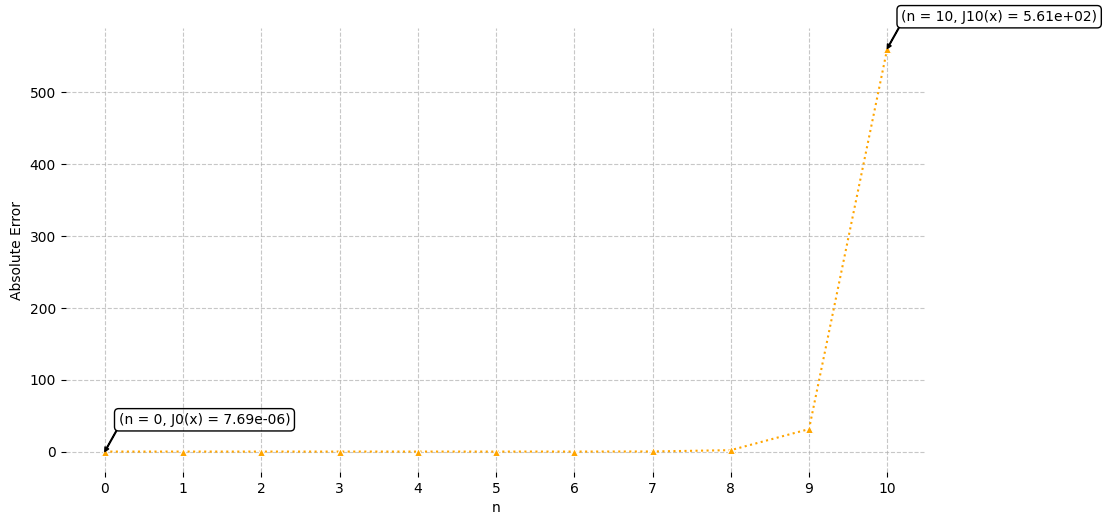
\includegraphics[width=\textwidth]{FW1.png} % Replace with your figure file
        \caption{Forward Error x = 1}
        \label{fig:fig1}
    \end{minipage}%
    \begin{minipage}{0.33\textwidth}

        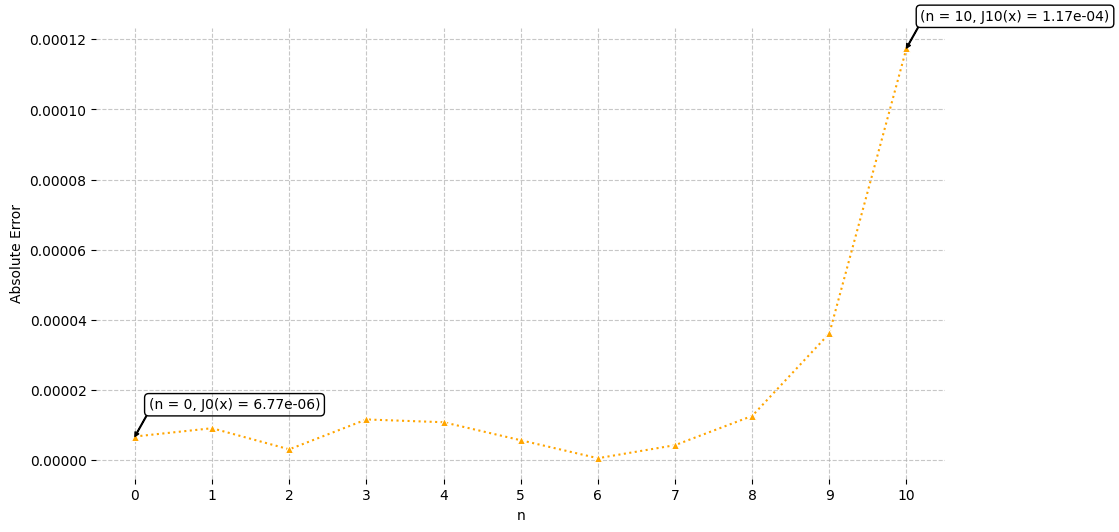
\includegraphics[width=\textwidth]{FW5.png} % Replace with your figure file
        \caption{Forward Error x = 5}
        \label{fig:fig2}
    \end{minipage}%
    \begin{minipage}{0.33\textwidth}
        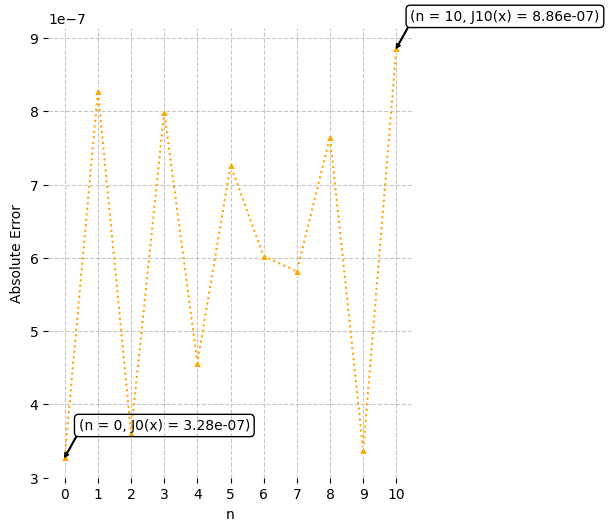
\includegraphics[width=\textwidth]{FW50.png} % Replace with your figure file
        \caption{Forward Error x = 50}
        \label{fig:fig3}
    \end{minipage}
\end{figure}

\textbf{Observations:} \\ 
1. From Figure 1, The error growth for x = 1 for forward pass is exponential.  The error in forward pass grew from order of $10^{-6}$ to order of $10^{2}$. \\ \\ 
2. From Figure 2, The error growth for x = 5 for forward pass seems to be exponential at around from n = \{6 to 10\}. The error in forward pass grew from order of $10^{-6}$ to order of $10^{-4}$. \\ \\ 
3. From Figure 3, The error growth for x = 50 is juggling randomly (not exponential) for forward pass. The error in forward pass is maintained in order of $10^{-7}$.
\\ \\ 
\textbf{Explanations:}
\\ \textit{Observation 1:} For $x=1$, from Table 5, we can see the $\beta \geq 2$ for all iterations, hence the error is increasing exponentially across the whole forward pass in Figure 1.
\\ \\ \textit{Observation 2:} For $x=5$, from Table 5, we can see that $\beta \geq 2$ for all values of $n \ \epsilon \ \{6,7,8,9,10\}$. Hence the error increases exponentially from $n = 6 \ to \ 10$ and the rest is non-exponential in Figure 2.
\\ \\ \textit{Observation 3:} For $x=50$, from Table 5, we can see that $\beta < 2$ for all iterations. Hence the error is juggling randomly (not exponential) in Figure 3.





\end{question}


\begin{question}{Q2 Compute the recursion backward, i.e. start with $J_{10}(x)$ from $J_9(x)$ compute $J_8(x)$. Again
use only the first 5 digits and for x = 1,5, and 50, how accurate is $J_0(x)$ in this backward
approach ?. Compute both the absolute and relative errors of these values taking the
tabulated values (table-1) as truth. Is the last value computed by the recurrence relation
is having less or more error compared to the forward approach ?. [3 points]}
\textbf{Solution:} We will initialize the last two rows ( $J_{10}(x)$ and $J_9(x)$ ) from values from the table using only the first 5 digits and compute backward.
Iterative scheme rearranged for backward computation: 
\begin{equation}
    J_{n}(x) = \frac{2(n+1)}{x}J_{n+1}(x) - J_{n+2}(x)
    \label{eq:backward}
\end{equation}
    
Errors can be calculated similarly to Q1. \\

\textbf{\textit{Q ...Compute both the absolute and relative errors of these values taking the tabulated values
(table-1) as truth.... }}


\begin{table}[H]
\centering
\begin{tabular}{c c c c}
\hline
 & $J_{0}(1)$ & $J_{0}(5)$ & $J_{0}(50)$ \\
\hline
ActualValue    & $7.6519768656 \times 10^{-1}$ & $-1.7759677131 \times 10^{-1}$ & $5.5812327669 \times 10^{-2}$ \\
ComputedValue  & $7.6519036352 \times 10^{-1}$ & $-1.7759388559 \times 10^{-1}$ & $5.5807275575 \times 10^{-2}$ \\
AbsoluteError  & $7.3230350601 \times 10^{-6}$ & $2.8857199839 \times 10^{-6}$ & $5.0520941498 \times 10^{-6}$ \\
RelativeError  & $9.5701217983 \times 10^{-6}$ & $-1.6248718727 \times 10^{-5}$ & $9.0519323611 \times 10^{-5}$ \\
\hline
\end{tabular}
\caption{Comparison of Actual, Computed Values, and Errors for $J_{0}(x)$ in forward computation.}
\label{tab:j0_values}
\end{table}



\begin{figure}[H]
    \begin{minipage}{0.33\textwidth}
        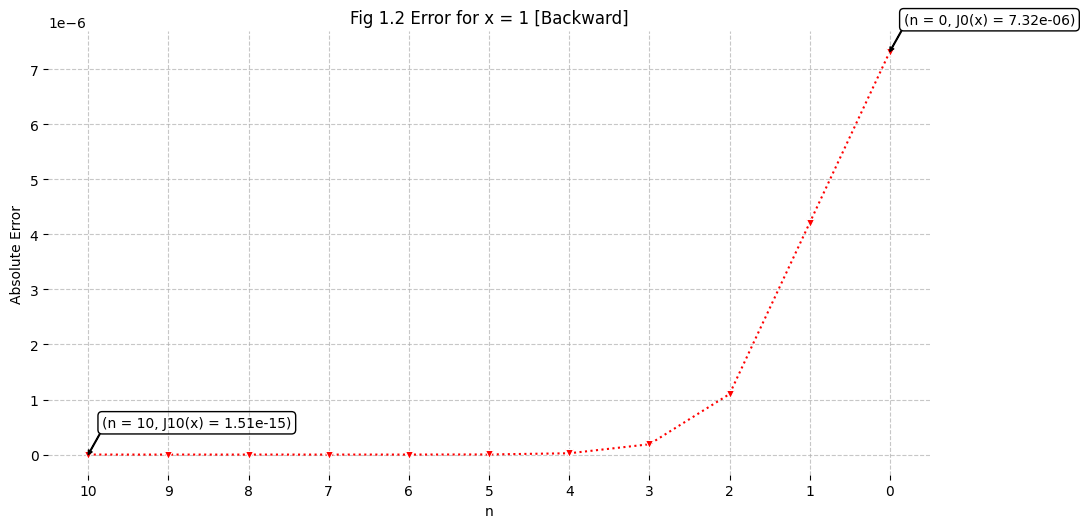
\includegraphics[width=\textwidth]{BW1.png} % Replace with your figure file
        \caption{Backward Error x = 1}
        \label{fig:fig1}
    \end{minipage}%
    \begin{minipage}{0.33\textwidth}

        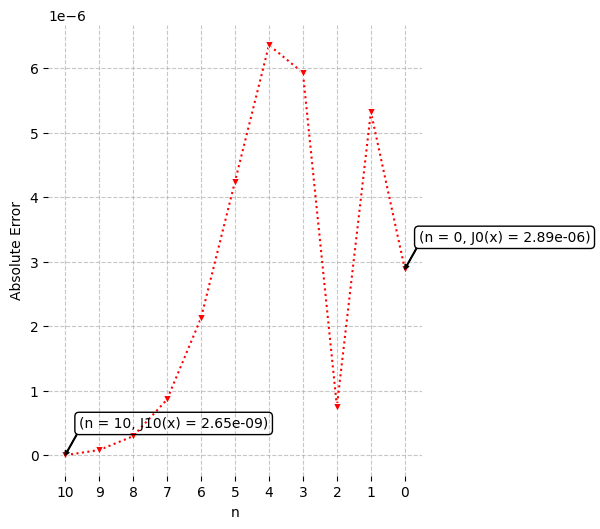
\includegraphics[width=\textwidth]{BW5.png} % Replace with your figure file
        \caption{Backward Error x = 5}
        \label{fig:fig2}
    \end{minipage}%
    \begin{minipage}{0.33\textwidth}
        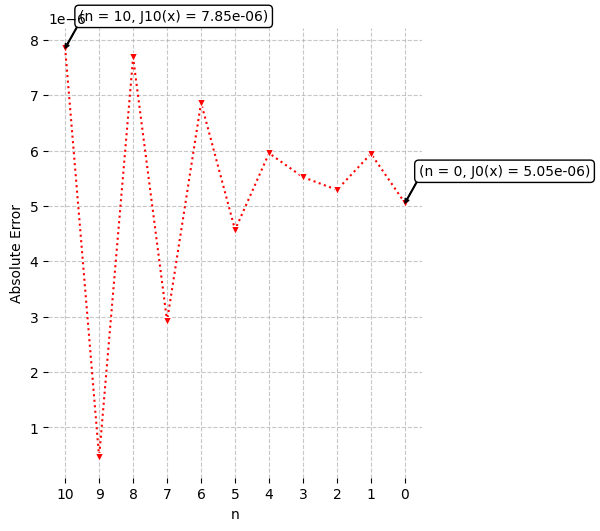
\includegraphics[width=\textwidth]{BW50.png} % Replace with your figure file
        \caption{Backward Error x = 50}
        \label{fig:fig3}
    \end{minipage}
\end{figure}

\textbf{Observations:} \\ 
4. From Figure 4, The error growth for x = 1 for backward pass is exponential. The error in backward pass grew from order of $10^{-15}$ to $10^{-6}$. \\ \\ 
5. From Figure 5, For backward pass, the error seems to be exponential till n = {10 to 4} and then juggling randomly (not exponential). The error in backward pass grew from order of $10^{-9}$ to $10^{-6}$. \\ \\ 
6. From Figure 6, The error growth for x = 50 is juggling randomly (not exponential) The error in backward pass is maintained in order of $10^{-6}$.


\textbf{Explanations:}
\\ \textit{Observation 4:} For $x=1$, from Table 6, we can see the $\beta \geq 2$ for all iterations, hence the error is increasing exponentially across the whole forward pass in Figure 4.
\\ \\ \textit{Observation 5:} For $x=5$, from Table 6, we can see that $\beta \geq 2$ for all values of $n \ \epsilon \ \{8,7,6,5,4\}$. Hence the error increases exponentially from $n = 10 \ to \ 4$ in and the rest is non-exponential in Figure 5.
\\ \\ \textit{Observation 6:} For $x=50$, from Table 6, we can see that $\beta < 2$ for all iterations. Hence the error is juggling randomly (not exponential) in Figure 6. \\

\textbf{\textit{Q: ...Is the last value computed by the recurrence relation having less or more error compared to the forward approach?}}

\begin{table}[H]
\centering
\begin{tabular}{c c c c c}
\hline
 & \textbf{Direction} & $J_{0}(1)$ & $J_{0}(5)$ & $J_{0}(50)$ \\
\hline
\textbf{AbsoluteError} & Backward  & $7.3230350601 \times 10^{-6}$ & $2.8857199839 \times 10^{-6}$ & ${5.0520941498 \times 10^{-6}}_M$ \\
\textbf{RelativeError}  & Backward & $9.5701217983 \times 10^{-6}$ & $-1.6248718727 \times 10^{-5}$ & ${9.0519323611 \times 10^{-5}}_M$ \\
\hline
 & Direction & $J_{10}(1)$ & $J_{10}(5)$ & $J_{10}(50)$ \\
\hline
\textbf{AbsoluteError} & Forward & ${5.6055331000 \times 10^{2}}_M$   & ${1.1745331430 \times 10^{-4}}_M$ & $8.8613829735 \times 10^{-7}$ \\
\textbf{RelativeError} & Forward & ${2.1308830203 \times 10^{12}}_M$  & ${8.0019827270 \times 10^{-2}}_M$ & $-7.7835313005 \times 10^{-6}$ \\
\hline
\end{tabular}
\caption{Comparison of errors in last iteration for Forward and Backward computation. Max values are marked with subscript $_M$.}
\label{tab:j0_values}
\end{table}

From Table 4, it is clear that the forward approach has more absolute and relative error for $x = 1$ and $x = 5$ whereas the backward approach has more relative and absolute error for $x=50$.


\end{question}

\begin{question}{Q3 Explain your finding. Can the error propagation be formally analyzed using the difference
equation analysis we performed in class? Can the error behavior be understood by this
analysis ?. Defend your answer to these questions. In case your answers are yes, do the
analysis. If the answer is no, how will you explain the error propagation ?. [4 points]}

\textbf{Solution:}
The error behavior can be analyzed using difference equation analysis. 

We know that to find the class of error growth, we have to write the iterative scheme. 

The forward scheme is given by $$J_{i}(x) = \frac{2(i-1)}{x}J_{i-1}(x) - J_{i-2}(x)$$

Now let us assume that the $\frac{2(i-1)}{x}$ is a constant represented by $\beta$. Our scheme then becomes: 

\begin{equation}
    J_{i}(x) = \beta J_{i-1}(x) - J_{i-2}(x)
    \label{eq:beta}
\end{equation}

Where $\beta$ varies with the input x. We can calculate the maximum and minimum values of $\beta$ to get some intuition about the errors.

As discussed in class, we cannot represent the numbers to their exact precision in computer. Let $\hat{J}_{i}(x)$ represent the representation we can have in our computers.

\begin{equation}
\hat{J}_{i}(x) = \beta \hat{J}_{i-1}(x) - \hat{J}_{i-2}(x)
\label{eq:betahat}
\end{equation}
Subtracting \eqref{eq:betahat} from \eqref{eq:beta} we get: $$e_{i}(x) = \beta e_{i-1}(x) - e_{i-2}(x)$$

Now, let's assume the error class is exponential

$$e_n \propto k^n \\ \implies k^i = \beta \cdot k^{i-1} - k^{i-2}   \\   \implies k^i - \beta \cdot k^{i-1} + k^{i-2} = 0   \\   \implies k^{i - 2} \left( k^2 - \beta k + 1 \right) = 0  \\ $$

$$\implies k = \frac{\beta \pm \sqrt{\beta^2 - 4}}{2}$$

Since $\beta > 0$, the roots of the equation will be real only if $ \beta \geq 2$, which is also the condition for which the error growth will be exponential as:

$$k_1 = \frac{\beta + \sqrt{\beta^2 - 4}}{2} \ and \ k_2 = \frac{\beta - \sqrt{\beta^2 - 4}}{2}$$
$$\epsilon_n =  C_1 \cdot k_1^n + C_2 \cdot k_2^n$$
$$since \ k_2 \leq 1 \ and \ k_1 \geq 1 \ \forall \  \beta \geq 2$$



For backward computation, we can use the same scheme except for the following changes: $$\epsilon_{n} \propto k^{10-n}$$

$$ e_{i}(x) = \beta e_{i+1}(x) - e_{i+2}(x)$$
$$\implies k^{10-i} = \beta \cdot k^{10-i-1} - k^{10-i-2}   \\   \implies k^{10- i - 2} \left( k^2 - \beta k + 1 \right) = 0  \\ $$

$$\implies k = \frac{\beta \pm \sqrt{\beta^2 - 4}}{2}$$

Which gives us the same condition $\beta \geq 2$. 

Now, we will calculate the values of $\beta$ that we will get for both forward and backward pass in an attempt to justify our claims. 


\begin{table}[H]
    \centering
    \begin{minipage}{0.45\textwidth}
        \centering
        \begin{tabular}{c c c c}
        \hline
        $n$ & $J_{n}(1)$ & $J_{n}(5)$ & $J_{n}(50)$ \\
        \hline
        2  & $\textbf{2.00}_e$ & {0.40} & {0.04} \\
        3  & $\textbf{4.00}_e$ & {0.80} & {0.08} \\
        4  & $\textbf{6.00}_e$ & {1.20} & {0.12} \\
        5  & $\textbf{8.00}_e$ & {1.60} & {0.16} \\
        6  & $\textbf{10.00}_e$ & $\textbf{2.00}_e$ & {0.20} \\
        7  & $\textbf{12.00}_e$ & $\textbf{2.40}_e$ & {0.24} \\
        8  & $\textbf{14.00}_e$ & $\textbf{2.80}_e$ & {0.28} \\
        9  & $\textbf{16.00}_e$ & $\textbf{3.20}_e$ & {0.32} \\
        10 & $\textbf{18.00}_e$ & $\textbf{3.60}_e$ & {0.36} \\
        \hline
        \end{tabular}
        \caption{Forward values}
        \label{tab:forward_values}
    \end{minipage}%
    \begin{minipage}{0.45\textwidth}
        \centering
        \begin{tabular}{c c c c}
        \hline
        $n$ & $J_{n}(1)$ & $J_{n}(5)$ & $J_{n}(50)$ \\
        \hline
        8  & $\textbf{18.00}_e$ & $\textbf{3.60}_e$ & {0.36} \\
        7  & $\textbf{16.00}_e$ & $\textbf{3.20}_e$ & {0.32} \\
        6  & $\textbf{14.00}_e$ & $\textbf{2.80}_e$ & {0.28} \\
        5  & $\textbf{12.00}_e$ & $\textbf{2.40}_e$ & {0.24} \\
        4  & $\textbf{10.00}_e$ & $\textbf{2.00}_e$ & {0.20} \\
        3  & $\textbf{8.00}_e$ & {1.60} & {0.16} \\
        2  & $\textbf{6.00}_e$ & {1.20} & {0.12} \\
        1  & $\textbf{4.00}_e$ & {0.80} & {0.08} \\
        0  & $\textbf{2.00}_e$ & {0.40} & {0.04} \\
        \hline
        \end{tabular}
        \caption{Backward values}
        \label{tab:backward_values}
    \end{minipage}
\end{table}

In Table 5 and Table 6, the values at which the growth will be exponential $\beta \geq 2$ are boldened and marked with subscript $_e$. \\ \\
These $\beta$ values are used to explain \textit{Observations 1-6} in \textbf{Q1} and \textbf{Q2} in the corresponding \textit{Explanations} section.



\end{question}

\begin{question} {CODE (Python)}
\lstinputlisting{Homework-1.py}
\end{question}
\end{document}


% \begin{question}{Problem 2 (multi-part example, and large numbers)}

% \begin{part}

% \textbf{Answer:} \fbox{$20! \cdot \binom{13}{5} \approx 3.131 \cdot 10^{21}$}

% (Please give the raw formula you used, \textbf{and} its value, possibly in scientific notation if it is too
% large).


% \textbf{Explanation:}

% Explain here.
% \end{part}

% \begin{part}

% \textbf{Answer:} \fbox{$answer$}

% \textbf{Explanation:} 

% Explain here.

% \end{part}

% \end{question}
% \begin{question}{Problem 3 (proof problem example)} 

% \textbf{(Short way)}

% You can use the \textbf{align*} environment to align a proof or
% calculation. Example below: 

% \begin{align*}
%     \P(E|F) &= \dfrac{\P(E \cap F)}{\P(F)}     & \text{(def of conditional probability)} \\
%             &= \dfrac{\P(F|E) \P(E)}{\P(F)}    & \text{(chain rule)}
% \end{align*}


% \textbf{How did I produce that?} The ``align*'' environment produces a table structure. You use \& to go to the next ``column'', and \text{\textbackslash \textbackslash} to start a new line. The whitespaces in the .tex document were not necessary. \\

% \textbf{(Long way)}

% First, by the chain rule, we have
% $$\P(E|F) \P(F) = \P(E \cap F)$$

% Switching the roles of $E$ and $F$ gives
% $$\P(F|E) \P(E) = \P(F \cap E)$$

% Since $\P(E \cap F) = \P(F \cap E)$, we can set them equal to get
% $$\P(E|F) \P(F) = \P(F|E) \P(E)$$

% But dividing by $\P(F) > 0$ gives Bayes Theorem
% $$\P(E|F) = \dfrac{\P(F|E) \P(E)}{\P(F)}$$
% \end{question}

% \begin{question}{Problem 4 (Calculus notation)}
% \begin{part} The syntax for integrals, summations, etc is a bit clunky but should be intuitive.

% $$ \int_{a}^{b}{f(x)dx} $$

% $$ \sum_{i=1}^{n} X_i $$

% $$ \prod_{i=1}^{n} \P(x_i | \theta) $$

% \end{part}
% \begin{part} Partial derivatives:
% $$ \dfrac{\partial}{\partial \theta} L(x_1, x_2, \dots x_n | \theta) = 2x$$

% \end{part}
% \end{question}


